\documentclass[class=article, crop=false, 12pt]{standalone}
\usepackage[subpreambles=true]{standalone}
\usepackage{../.common/common}


\author{Tony Shing}
%\pretitle{Supplementary}

\topic{Note 08 (Thermodynamics)}
\title{Thermodynamics \nth{1} Law}

\version{2025} % leave blank for omitting

\begin{document}

\maketitle


\begin{overview}
    \begin{itemize}
        \item Terminologies: State functions \& Processes
        \item Review the 4 most common thermal processes 
        $\bcase{
            &\text{Formula true for everything} \\ 
            &\text{Formula for ideal gas only}
        }$
        \item Calculation for thermal cycle, efficiency and COP
    \end{itemize}
\end{overview}


% content begins here
% Section %%%%%%%%%%%%%%%%%%%%%%%%%%%%%%%%%%%%%%%%%%%%%%%%%%%%
\section{Thermodynamics \nth{1} Law}

The thermodynamics \nth{1} law is essentially energy conservation.
\aleq{
    &&&&\var{Q} = \dd{U} + \var{W}  &&&&(\text{Physics convention})
}
\begin{itemize}
    \item $\var{Q} = $ Heat \cul[red]{input to} the system.
    \item $\dd{U} = $ Change in internal energy of the system.
    \item $\var{W} = $ Work done \cul[red]{by} the system.
\end{itemize}

\ul{Note:} The convention in Chemistry books are different from Physics books.
\aleq{
    &&&&\dd{U} = \var{Q} + \var{W}  &&&&(\text{Chemistry convention})
}
This is due to chemists refer $\var{W}$ as the work done \cul[red]{to} system,
so work done \cul[blue]{by} system is $\cul[blue]{-}\var{W}$.


%%%%%%%%%%%%%%
\subsection{Terminologies in Thermodynamics}

To deep dive into thermodynamics, 
here are some terminologies you must understand.

\begin{enumerate}
    \item \bf{\ul{State}}\\
    We describe a system in a "specific state" 
    if the system can be "well-distinguished" by a set of parameters.
    \begin{center}
            \red{\ul{\ul{Different parameters \quad$\Leftrightarrow$\quad Different states}}}
    \end{center}

    For example,
    \begin{itemize}
        \item \ul{Ideal gas system}\\
        Every possible state of a box of gas can be described solely by 3 parameters $(P,V,T)$.\\
        \gray{But only 2 of them are independent, because we have ideal gas law $PV=nRT$.}\\

        \item \ul{Mechanical system}\\
        Mechanical system must satisfy Newton's \nth{2} law - a \nth{2} order ODE
        - which the particle's motion is completely determined after knowing its initial position $(x,y,z)$ and velocity $(v_x,v_y,v_z)$, 
        6 parameters in total.\\
        \gray{To describe the state of a mechanical system with $N$ bodies, it takes $6N$ parameters.}

    \end{itemize}

    \vskip 1ex
    \item \bf{\ul{State Space}}\\
    The state space is an abstract representation of \cul[red]{the set of all possible states} using state parameters.
    
    \begin{center}
        \begin{minipage}{0.37\linewidth}
            \centering
            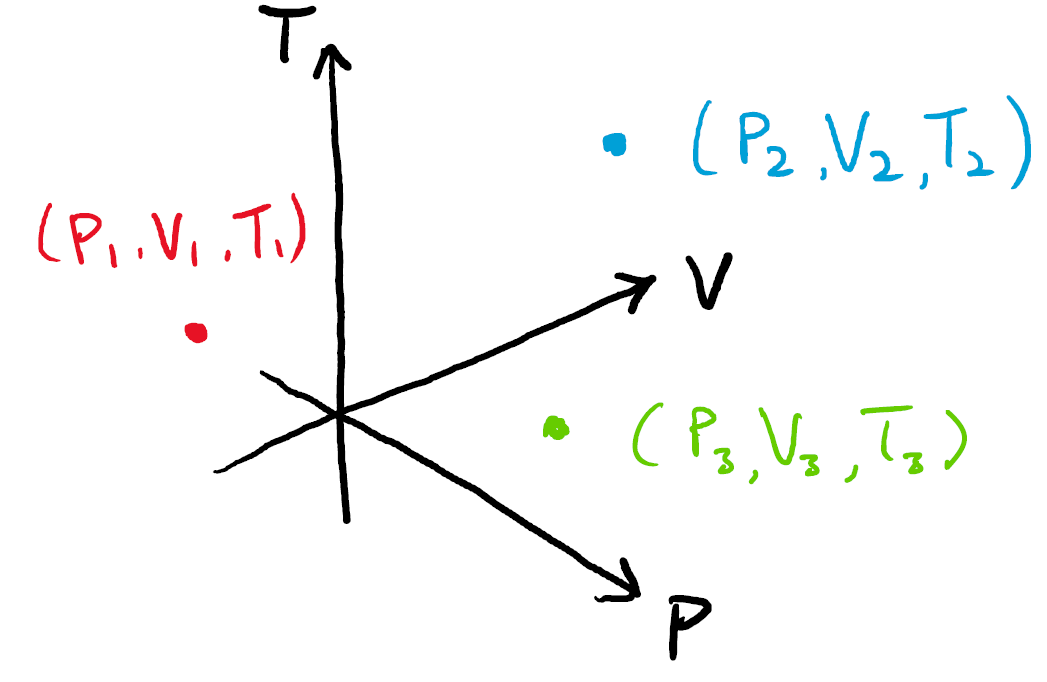
\includegraphics[width=\textwidth]{state_sp}
        \end{minipage}
        \begin{minipage}{0.6\linewidth}
            \centering
            Because ideal gas system only takes 3 parameters,\\ 
            we can draw it out as a 3D space,\\ 
            with each coordinate representing\\
            a possible state of the gas.
        \end{minipage}
    \end{center}

    \item \bf{\ul{Process}}\\
    It is the transition between states.
    If the state space can plotted out, 
    processes are the paths connecting different states.

    \begin{center}
        \begin{minipage}{0.25\linewidth}
            \centering
            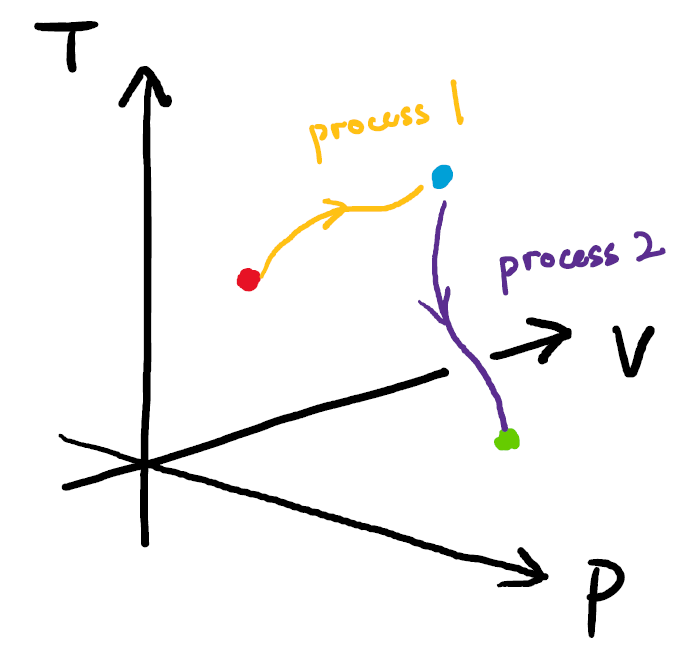
\includegraphics[width=\textwidth]{state_pro}
        \end{minipage}
        \hspace{0.05\textwidth}
        \begin{minipage}{0.6\linewidth}
            \centering
            For ideal gas, because only 2 of $(P,V,T)$ \\
            are independent,
            we can project the processes' path onto a 2D plane, 
            creating the P-V diagram\\
             (or P-T/V-T diagram).
        \end{minipage}
    \end{center}


    \item \bf{\ul{State Function}}\\
    State functions are functions that only take state parameters as inputs.
    \begin{center}
        \red{A state function's values are well-defined for every state.}
    \end{center}

    For example, for a scalar state function,
    we can draw it as a smooth height map:

    \begin{center}
        \begin{minipage}{0.4\linewidth}
            \centering
            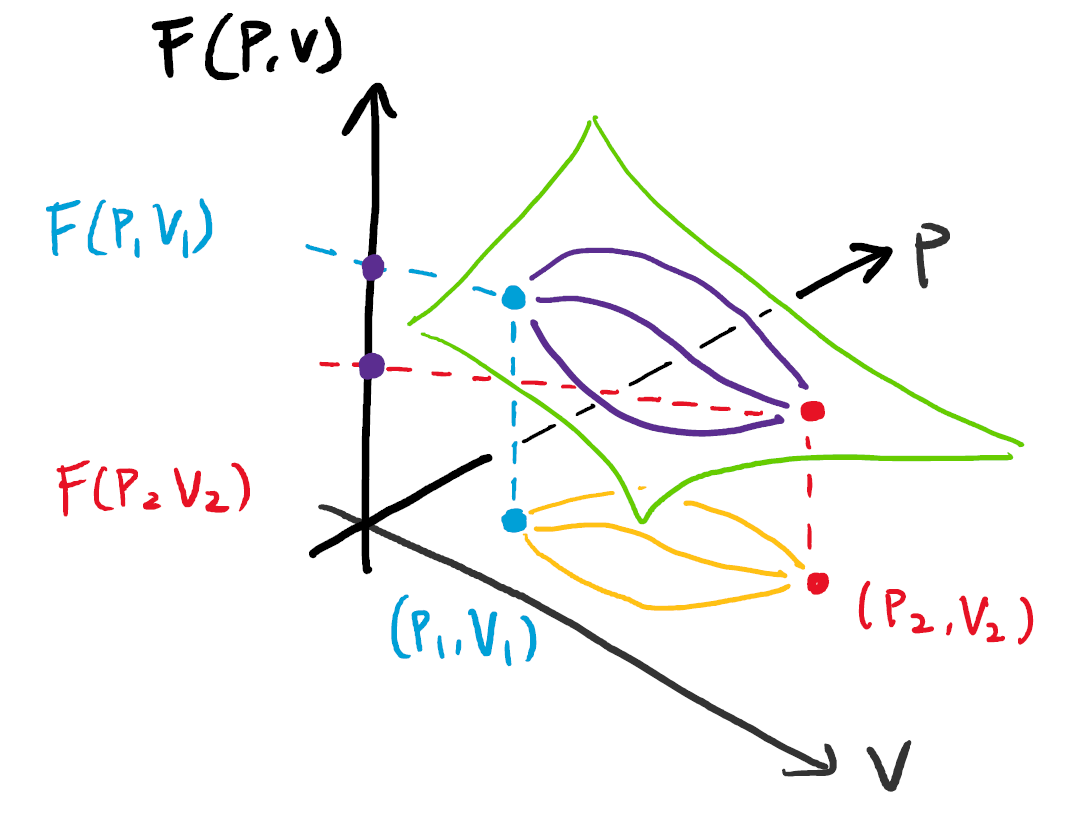
\includegraphics[width=\textwidth]{state_func1}
        \end{minipage}
        $\qquad\Rightarrow\qquad$
        \begin{minipage}{0.4\linewidth}
            \centering
            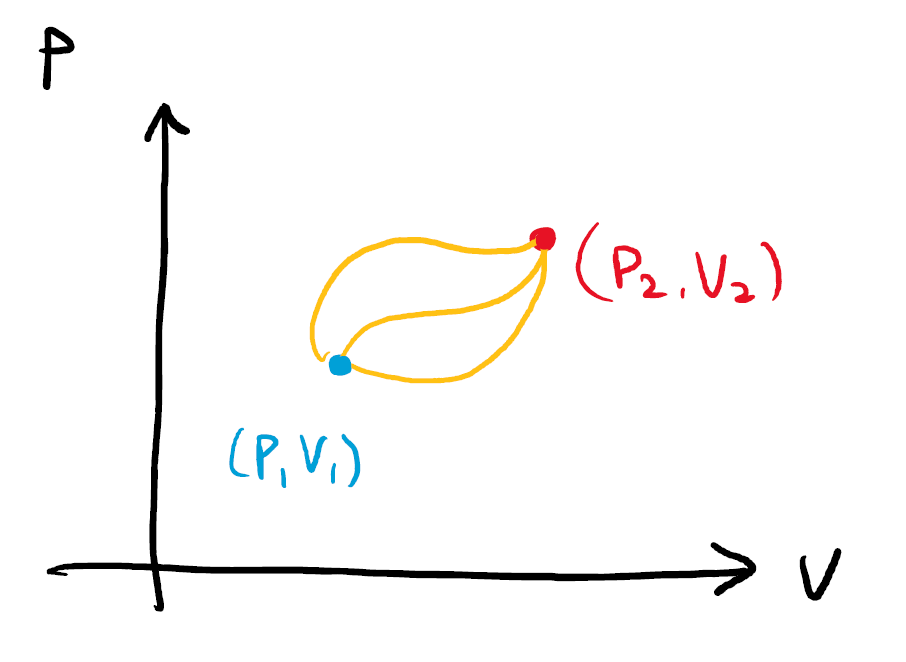
\includegraphics[width=\textwidth]{state_func2}
        \end{minipage}
    \end{center}

    You can think of a state function like some potential function.
    \aleq{
        \mstack{\text{Total change}\\\text{of }F(P,V,T)} 
        = \int_{\substack{\yellow{\text{Any process}}\\\blue{(P_1,V_1,T_1)}\to\red{(P_2,V_2,T_2)}}} \dd{F}
        = F(\red{P_2,V_2,T_2}) - F(\blue{P_1,V_1,T_1})
    }



\end{enumerate}

%%%%%%%%%%%%%%
\subsection{State Functions v.s. Non-State Functions}

Here are some examples of state function in thermodynamics:
\begin{itemize}
    \item \ul{The state parameters themselves} - you can always write something like $F(P,V,T)=P$.
    
    \item \ul{Internal energy} - such as potential energy and kinetic energy. 
    
    \begin{center}
        \begin{minipage}{0.12\linewidth}
            \centering
            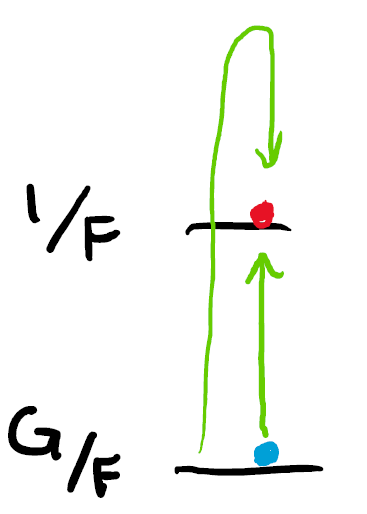
\includegraphics[width=\textwidth]{PE}
        \end{minipage}
        \begin{minipage}{0.7\linewidth}
            \centering
            Here the state parameter is the height.\\
            Change in PE only depends on initial and final height,
            independent of the path we take.
        \end{minipage}
    \end{center}

    \item \ul{Entropy} \gray{(Only in some situation)}
    
\end{itemize}

\vskip 1em
And here are some examples that are NOT state function in thermodynamics:
\begin{itemize}
    \item \ul{Work Done} \\
    By definition,
    \aleq{
        \Delta \text{(W.D.)} = \tkn{WD_P}{\cul[red]{P}}\cdot \tkn{WD_V}{\cul[blue]{\Delta V}}
    }
    \addArrow[red]{WD_P}{(-3ex,-3ex)}
    {\scriptsize $P$ is a state parameter\\[-0.8ex]\scriptsize No problem}
    {(0,-1ex)}{(-5ex,-1ex)}
    \addArrow[blue]{WD_V}{(3ex,-3ex)}
    {\scriptsize $\Delta V$ = \cul[blue]{\blue{Change}} of a state parameter\\[-0.8ex]\scriptsize NOT well-defined on a given state}
    {(0,-1ex)}{(8ex,-1ex)}

    \vskip 1.5em
    Because you cannot define work done with only one state, 
    it cannot be a state function. 
    In fact, we always visualize W.D. as the area under curve (= process!) in the P-V diagram,
    indicating that it is a property of a process.
    

    \begin{center}
        \begin{minipage}{0.3\linewidth}
            \centering
            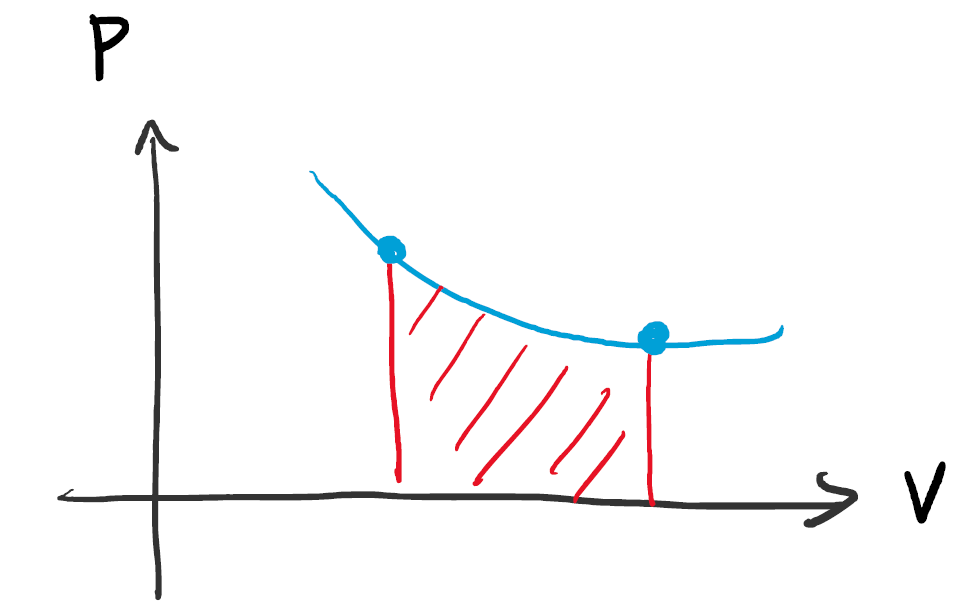
\includegraphics[width=\textwidth]{PV}
        \end{minipage}
        \hspace{0.02\textwidth}
        \begin{minipage}{0.6\linewidth}
            \aleq{
                \sum_{\text{segments }i} P_iV_i \sim \int_\text{process} P\dd{V} = \text{Area under curve}
            }
        \end{minipage}
    \end{center}

    \item \ul{Heat}\\
    According to the \nth{1} law,
    \aleq{
        \var{Q} = \tkn{H_U}{\cul[red]{\dd{U}}} + \tkn{H_W}{\cul[blue]{\var{W}}}
    }
    \addArrow[red]{H_U}{(-3ex,-3ex)}{\scriptsize State function}{(0,-1ex)}{(-2ex,0)}
    \addArrow[blue]{H_W}{(3ex,-3ex)}{\scriptsize Process dependent}{(0,-1ex)}{(2ex,0)}

    So heat must also depend on the process.

\end{itemize}

\begin{notation}[Side note:]
    Note the notation difference between $\dd{U}$ v.s. $\var{W},\var{Q}$:
    \begin{itemize}
        \item Change in state function $\Rightarrow$ Use \red{$\dd$} 
        \item Change in path dependent function $\Rightarrow$ Use \red{$\var$}
    \end{itemize}

    This is significant when doing (line) integral:
    \begin{itemize}
        \item \red{$\dd$} $\Rightarrow$ Independent of path. 
        Simply substract the initial value from final value.
        \aleq{
            \int \dd{U} = U_f - U_i
        }

        \item \red{$\var$} $\Rightarrow$ Path dependent.
        Must do the integral explicitly.
        \begin{itemize}
            \item Without knowing the given path, we must write $\displaystyle \int \red{\var}{W}, \int \red{\var}{Q}$
            \item After the path is known, we can write $\displaystyle \int_\blue{C} \red{\dd}{W}, \int_\blue{C} \red{\dd}{Q}$
        \end{itemize}
    \end{itemize}
\end{notation}

\vskip 1em
\linesep
% Section %%%%%%%%%%%%%%%%%%%%%%%%%%%%%%%%%%%%%%%%%%%%%%%%%%%%
\section{The 4 Most Common Processes}

\begin{notation}
    In the following section, I will stick to the colour scheme:
    \begin{itemize}
        \item \fcbox[red]{Red boxed} - True for any processes.
        \item \fcbox[blue]{Blue boxed} - Only true for ideal gas. Derivation requires ideal gas' properties.
    \end{itemize}
\end{notation}

\vskip 1em
Normally, thermodynamics texts only concern these 4 processes:
\begin{center}
    \begin{tabular}{c|c}
        Isovolumetric (Isochoric) & $V=$ const. \\
        \hline
        Isobaric & $P =$ const. \\
        \hline
        Isothermal & $T=$ const. \\
        \hline
        Adiabatic & $\var{Q} = 0$
    \end{tabular}
\end{center}

It is essential to find the $\dd{U}, \var{W}$ and $\var{Q}$ for each of the 4 process.
We can even promote the derivation to find them for arbituary processes.

%%%%%%%%%%%%%%
\subsection{Internal Energy}

As mentioned, internal energy is a state function - 
\red{change in internal energy is independent of process.}
So if the function form of $U$ is not known, we can only write
\aleq{
    \Acboxed[red]{
        \Delta U = U(P_2,V_2,T_2) - U(P_1,V_1,T_1)
    }
}

In case of ideal gas, 
the function form of $U$ is derived using kinetic theory:
\vskip 1em
\aleq{
    U(P,V,T) = \tkn{dof}{\frac{\cbox[blue]{i}}{2}}\tkn{U_ideal1}{\cul[green]{PV}} = \tkn{gas_law}{\frac{i}{2}\tkn{U_ideal2}{\cul[green]{nRT}}}
}
\addArrow[blue]{dof}{(0,3ex)}
{\scriptsize $i=$ degree of freedom}{(0,4ex)}
\addBelowArrow[green]{U_ideal1}{U_ideal2}{\scriptsize By ideal gas law}{-2ex}

Therefore,
\vskip -3ex
\aleq{
    \Acboxed[blue]{
        \Delta U = \frac{i}{2}(P_2V_2 - P_1V_1) = \frac{i}{2}nR\tkn{U_Tonly}{(\cul[green]{T_2-T_1})}
    }
}
\addArrow[green]{U_Tonly}{(0,-5ex)}{$U$ of ideal gas can be written as a function of only $T$!}{(0,-1ex)}


\vskip 2em
%%%%%%%%%%%%%%
\subsection{Isovolumetric Process (const. $V$)}

\begin{center}
    \begin{minipage}{0.3\linewidth}
        \centering
        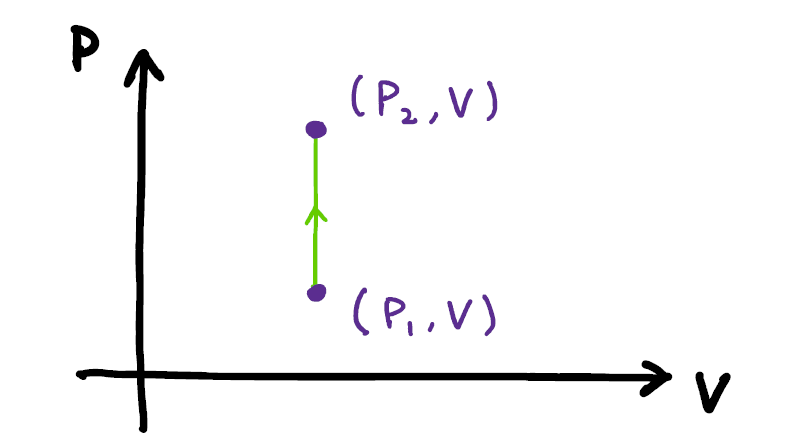
\includegraphics[width=\textwidth]{isoV}
    \end{minipage}
    \begin{minipage}{0.4\linewidth}
        \centering
        Always vertical line in PV diagram.
    \end{minipage}
\end{center}

\begin{enumerate}
    \item \ul{Work Done} \\
    By definition of the process, 
    \aleq{
        \Acboxed[red]{
            \int \var{W} = \int_{\yellow{\text{iso. }V}} \dd{W} 
            = \int_{\yellow{\text{iso. }V}} P\tkn{isoV_W}{\cul[red]{\dd{V}}} = 0
        }
    }
    \addArrow[red]{isoV_W}{(0,-5ex)}{$V$ cannot change}{(0,-0.8ex)}

    \item \ul{Heat} \\
    By \nth{1} law,
    \aleq{
        \var{Q} = \dd{U} + \ccancelto[red]{0}{\var{W}} = \dd{U}
    }
    So we can write 
    \aleq{
        \Acboxed[red]{
            \int \var{Q} = \int_{\yellow{\text{iso. }V}} \dd{Q} = \int \dd{U} = U_2 - U_1
        }
    }

    We can also define $C_V$, the \bf{heat capacity under constant volume}:
    \aleq{
        \Acboxed[red]{
            \int_{\yellow{\text{iso. }V}} \dd{Q} = \int C_\yellow{V} \dd{T}
            \qquad\Leftrightarrow\qquad
            C_\yellow{V}(T) = \qty(\dvv{Q}{T})_\yellow{\text{iso. }V} = \qty(\dvv{U}{T})
        }
    }

    When the internal energy of ideal gas law is given,
    \aleq{
        U_2-U_1 &= \frac{i}{2}(P_2V_2 - P_1V_1) = \frac{i}{2}nR(T_2-T_1) \\
        &= \frac{i}{2}V(P_2-P_1) 
    }
    so we have
    \aleq{
        \Acboxed[blue]{
            \int_{\yellow{\text{iso. }V}} \dd{Q} \equiv U_2-U_1 = \frac{i}{2}V(P_2-P_1) = \frac{i}{2}nR(T_2-T_1)
        }
    }
    and
    \aleq{
        \Acboxed[blue]{
            C_\yellow{V}(T) \equiv \qty(\dvv{U}{T}) = \frac{i}{2}nR = (\text{Constant})
        }
    }

\end{enumerate}

\vskip 2em
%%%%%%%%%%%%%%
\subsection{Isobaric Process (const. $P$)}

\begin{center}
    \begin{minipage}{0.3\linewidth}
        \centering
        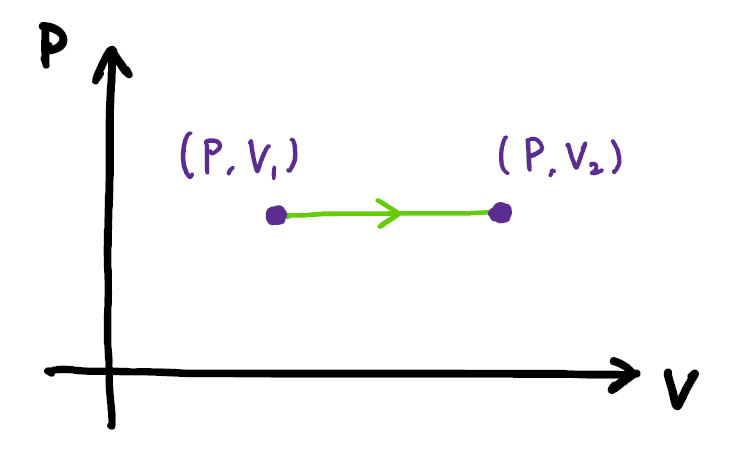
\includegraphics[width=\textwidth]{isoP}
    \end{minipage}
    \begin{minipage}{0.4\linewidth}
        \centering
        Always horizontal line in PV diagram.
    \end{minipage}
\end{center}

\begin{enumerate}
    \item \ul{Work Done}\\
    By definition of work done,
    \aleq{
        \Acboxed[red]{
            \int \var{W} = \int_\yellow{\text{iso. }P} \dd{W}
            = \int P\dd{V} = \tkn{isoP_W}{\cul[red]{P}}\int \dd{V} = P(V_2-V_1)
        }
    }
    \addArrow[red]{isoP_W}{(0,-4ex)}{$P$=constant}{(0,-0.8ex)}

    Substituting ideal gas law, we can also write
    \aleq{
        \Acboxed[blue]{
            \int_\yellow{\text{iso. }P} \dd{W} = nR(T_2-T_1)
        }
    }

    \item \ul{Heat}\\
    By \nth{1} law,
    \aleq{
        \var{Q} &= \dd{U} + \var{W}\\
        \Acboxed[red]{
            \int_\yellow{\text{iso. }P} \dd{Q} &= (U_2-U_1) + P(V_2-V_1)
        }
    }

    We can also define $C_P$, the \bf{heat capacity under constant pressure}:
    \aleq{
        \Acboxed[red]{
            \int_{\yellow{\text{iso. }P}} \dd{Q} = \int C_\yellow{P} \dd{T}
            \qquad\Leftrightarrow\qquad
            C_\yellow{P}(T) = \qty(\dvv{Q}{T})_\yellow{\text{iso. }P} = \qty(\dvv{U}{T}) + P\qty(\dvv{V}{T})
        }
    }

    Then for ideal gas,
    \aleq{
        \int_\yellow{\text{iso. }P} \dd{Q} &\equiv (U_2-U_1) + P(V_2-V_1) \\
        &= \frac{i}{2}P(V_2-V_1) + P(V_2-V_1) \\
        \Acboxed[blue]{
            \int_\yellow{\text{iso. }P} \dd{Q} &= \frac{i+2}{2}P(V_2-V_1) = \frac{i+2}{2}nR(T_2-T_1)
        }
    }

    and 
    \aleq{
        \Acboxed[blue]{
            C_\yellow{P}(T) \equiv \qty(\dvv{U}{T}) + P\qty(\dvv{P}{T})= \frac{i+2}{2}nR = (\text{Constant})
        }
    }
\end{enumerate}

\vskip 1em
%%%%%%%%%%%%%%
\subsection{Isothermal Process (const. $T$)}

\begin{center}
    \begin{minipage}{0.3\linewidth}
        \centering
        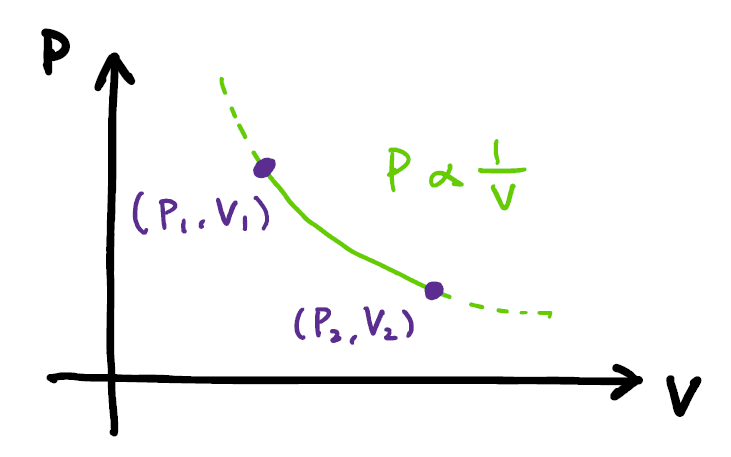
\includegraphics[width=\textwidth]{isoT}
    \end{minipage}
    \begin{minipage}{0.4\linewidth}
        \centering
        They look like this \red{only for ideal gas!}
    \end{minipage}
\end{center}

\begin{enumerate}
    \item \ul{Work Done}\\
    We are unable to reduce the form $\cbox[red]{\displaystyle \int_\yellow{\text{iso. }T}\var{W} = \int P\dd{V}}$ 
    unless we know what is the relation between $P$ and $V$ of the material.\\

    For ideal gas, this relation is already known: $\displaystyle P = \frac{nRT}{V}$.
    Then the integral becomes
    \aleq{
        \Acboxed[blue]{
            \int_\yellow{\text{iso. }T} \var{W} 
            = \int \frac{nRT}{V}\dd{V} 
            = nR\tkn{isoT}{\cul[blue]{T}}\int \frac{\dd{V}}{V} 
            = nRT\ln\qty(\frac{V_2}{V_1})
        }
    }
    \addArrow[blue]{isoT}{(0,-5ex)}{$T=$ constant}{(0,-1ex)}

    \item \ul{Heat}\\
    Even with \nth{1} law, again, we cannot reduce the form $\cbox[red]{\displaystyle \int_\yellow{\text{iso. }T}\var{Q} = (U_2 - U_1) + \int P\dd{V}}$
    unless we know what is the relation between $P$ and $V$ of the material.

    For ideal gas, because its internal energy can be written in a form that only has $T$,
    \aleq{
        \int \dd{U} = \frac{i}{2}nR(T_2-T_1) = 0
    }

    Then 
    \aleq{
        \Acboxed[blue]{
            \int_\yellow{\text{iso. }T} \var{Q} 
            = 0 + \int_\yellow{\text{iso. }T} \var{W} 
            = nRT\ln\qty(\frac{V_2}{V_1})
        }
    }

\end{enumerate}

%%%%%%%%%%%%%%
\subsection{Adiabatic Process ($\var{Q}=0$)}

\begin{center}
    \begin{minipage}{0.3\linewidth}
        \centering
        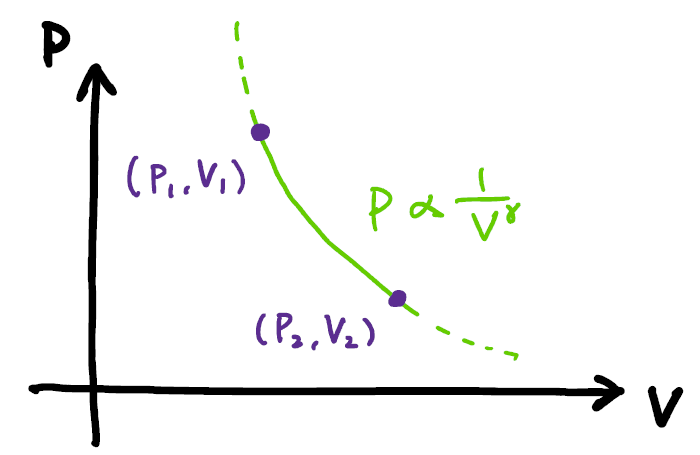
\includegraphics[width=\textwidth]{adiabatic}
    \end{minipage}
    \begin{minipage}{0.4\linewidth}
        \centering
        \red{$\gamma$ is different for different material.}
    \end{minipage}
\end{center}

\begin{enumerate}
    \item \ul{Heat}\\
    By definition of the process, 
    there must be no energy exchange in the form of heat.
    \aleq{
        \Acboxed[red]{
            \var{Q} = 0
        }
    }


    \item \ul{Work Done}\\
    By \nth{1} law, 
    \vskip -2em
    \aleq{
        \var{Q} &= \dd{U} + \var{W} \\
        \Acboxed[red]{
            \var{W} &= - \dd{U}
        }
    }


    \item \ul{Adiabatic Relation}\\
    Because all $P,V,T$ of initial and final states in an adiabatic process are different, 
    we need to derive the equation of the line connecting the two states.
    The set of equations of the lines is called \bf{adiabatic relation}.\\

    The relation depends on the form of $U(P,V,T)$.
    We always start the derivation from
    \aleq{
        \Acboxed[red]{
            -\dd{U} = \var{W} = P\dd{V}
        }
    }

    For ideal gas, $U = \frac{i}{2}PV$, 
    so $\dd{U} = \frac{i}{2}(P\dd{V} + V\dd{P})$.
    Substitute to above,
    \aleq{
        -\frac{i}{2}(P\dd{V}+V\dd{P}) &= P\dd{V} \\
        -\frac{i}{2} V\dd{P} &= \frac{i+2}{2}P\dd{V}\\
        \inv{P}\dd{P} &= -\frac{i+2}{i}\inv{V}\dd{V}\\
        \int \inv{P}\dd{P} &= -\frac{i+2}{i} \int \inv{V}\dd{V}\\
        \ln{P} &= -\frac{i+2}{i} \ln{V} + (\text{Constant})\\
        \ln\qty(PV^{\frac{i+2}{i}}) &= (\text{Constant}) \\
        \Acboxed[blue]{
            PV^{\frac{i+2}{i}} &= (\text{Constant})
        }
    }

    In general, adiabatic relation of common materials would have the form $\cbox[red]{PV^\gamma = (\text{constant})}$,
    where the index $\gamma$ is called \bf{adiabatic constant}. \\

    For ideal gas, $\cbox[blue]{\gamma = \frac{i+2}{i} = \frac{C_P}{C_V}}$.
    However this value \cul[red]{does NOT apply to every material}. 
    To some material, its adiabatic "constant" may not even be a constant.  


\end{enumerate}

\newpage
%%%%%%%%%%%%%%
\subsection{Summary}

Summarizing all useful formula under a table:

\begin{center}
    \begin{tabular}{c|c|c|c}
        & \makecell{$U$ \\ \green{is a state function}} 
        & \makecell{$W$ \\ \green{derive from definition:}\\\green{$\var{W} = P\dd{V}$}} 
        & \makecell{$Q$ \\ \green{derive by \nth{1} law:}\\\green{$\var{Q} = \dd{U} + \var{W}$}}
        \\[1em]
        \hline
        Iso. V 
        &
        $\begin{aligned} 
            & \,\cbox[red]{U(P_2,V,T_2) - U(P_1,V,T_1)}\\
            =& \,\cbox[blue]{\frac{i}{2}V(P_2-P_1)}\\
            =& \,\cbox[blue]{\frac{i}{2}nR(T_2-T_1)}
        \end{aligned}$
        & 0
        & 
        \makecell{
            \phantom{\scriptsize abc}\\
            $\begin{aligned}
                &= \cbox[red]{\int \dd{U} + 0}\\
                &= \cbox[red]{\int C_V \dd{T}} \\
                &= \cbox[blue]{\cub[blue]{\frac{i}{2}nR}{C_V}(T_2-T_1)}
            \end{aligned}$\\
            \phantom{\scriptsize abc}
        }
        \\[1em]
        \hline
        %
        Iso. P
        & 
        $\begin{aligned} 
            & \,\cbox[red]{U(P,V_2,T_2) - U(P,V_2,T_1)}\\
            =& \,\cbox[blue]{\frac{i}{2}P(V_2-V_1)}\\
            =& \,\cbox[blue]{\frac{i}{2}nR(T_2-T_1)}
        \end{aligned}$
        & 
        $\begin{aligned}
            & \,\cbox[red]{P(V_2-V_1)} \\
            =& \,\cbox[blue]{nR(T_2-T_1)}
        \end{aligned}$
        & 
        \makecell{
            \phantom{\scriptsize abc}\\
            $\begin{aligned}
                &= \cbox[red]{\int \dd{U} + \int \var{W}}\\
                &= \cbox[red]{\int C_P \dd{T}} \\
                &= \cbox[blue]{\cub[blue]{\frac{i+2}{2}nR}{C_P}(T_2-T_1)}
            \end{aligned}$\\
            \phantom{\scriptsize abc}\\
        }
        \\[2em]
        \hline
        %
        Iso. T
        & 
        $\begin{aligned} 
            & \,\cbox[red]{U(P_1,V_2,T) - U(P_1,V_2,T)}\\
            =& \,\cbox[blue]{0}\\
        \end{aligned}$
        & 
        \makecell{
            \phantom{\scriptsize abc}\\
            $\begin{aligned}
                & \,\cbox[red]{\int P\dd{V}} \\
                =& \,\cbox[blue]{nRT\ln\qty(\frac{V_2}{V_1})}
            \end{aligned}$\\
            \phantom{\scriptsize abc}
        }
        & 
        $\begin{aligned}
            &= \cbox[red]{\int \dd{U} + \int \var{W}}\\
            &= \cbox[blue]{nRT\ln\qty(\frac{V_2}{V_1})}
        \end{aligned}$
        \\[1em]
        \hline
        Adiabatic
        & 
        \makecell{
            \phantom{\scriptsize abc}\\
            $\begin{aligned} 
                & \,\cbox[red]{U(P_2,V_2,T_2) - U(P_1,V_1,T_1)}\\
                =& \,\cbox[blue]{\frac{i}{2}(P_2V_2-P_1V_2)}\\
                =& \,\cbox[blue]{\frac{i}{2}nR(T_2-T_1)}
            \end{aligned}$\\
            \phantom{\scriptsize abc}
        }
        
        & 
        $\begin{aligned} 
            &= \cbox[red]{-\dd{U}}\\
            &= \cbox[blue]{-\frac{i}{2}(P_2V_2-P_1V_2)}\\
            &= \cbox[blue]{-\frac{i}{2}nR(T_2-T_1)}
        \end{aligned}$
        & 0
    \end{tabular}
\end{center}




\linesep
\newpage
% Section %%%%%%%%%%%%%%%%%%%%%%%%%%%%%%%%%%%%%%%%%%%%%%%%%%%%
\section{Solving Thermal Cycle}

In this section, 
we will deal with one of the basic but extremely common problem in thermodynamics - 
given an arbituary thermal cycle, 
derive the formula of effciency / coefficient of performance (COP). 

\begin{center}
    \begin{minipage}{0.2\linewidth}
        \centering
        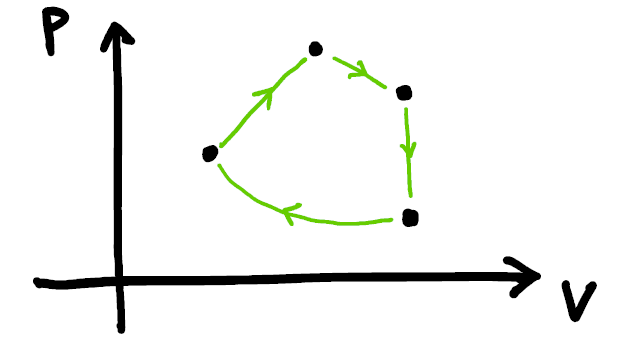
\includegraphics[width=\textwidth]{any_cycle}
    \end{minipage}
    $\qquad\Rightarrow\qquad$
    \begin{minipage}{0.25\linewidth}
        \centering
        Efficiency? COP?
    \end{minipage}
\end{center}


In general, you can follow these steps:
\begin{notation}[]
    \begin{enumerate}
        \item Write down the relation of $P,V,T$ between initial/final states of each process.
        \item Write down the $\dd{U}, \var{W}, \var{Q}$ for each process. 
        \item Identify if the $\var{Q}$ of each process is an input or output.
        \item Calculate efficiency / COP according to the signs of $\var{Q}$.
    \end{enumerate}
\end{notation}

\vskip 3em
\begin{example}
    A thermal cycle of \cul[blue]{ideal gas} with all 4 kinds processes.
    
    \begin{center}
        \begin{minipage}{0.4\linewidth}
            \begin{enumerate}
            \item Iso. T (expansion)
            \item Adiabatic (expansion)
            \item Iso. P (contraction)
            \item Iso. V
        \end{enumerate}
        \end{minipage}
        \hspace{0.05\textwidth}
        \begin{minipage}{0.3\linewidth}
            \centering
            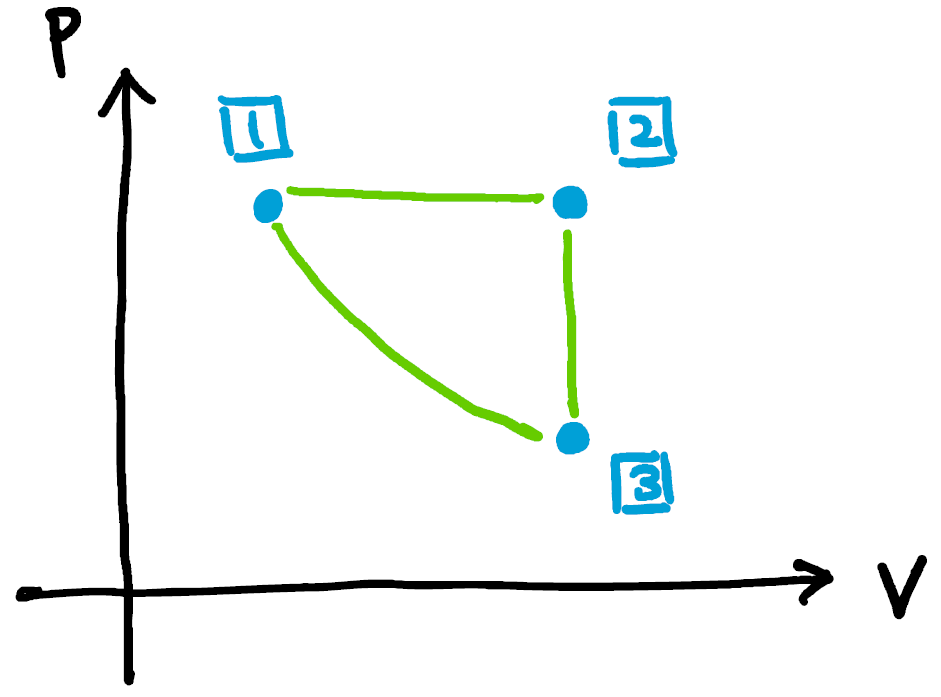
\includegraphics[width=\textwidth]{rand_cycle}
        \end{minipage}
    \end{center}

    \vskip 1em
    \begin{enumerate}
        \item Write down the relations of $P,V,T$ between initial/final states of each process.
        \begin{center}
            \begin{minipage}{0.65\linewidth}
                \centering
                \begin{tabular}{>{\centering\arraybackslash}m{3cm} >{\centering\arraybackslash}m{3cm} >{\centering\arraybackslash}m{3cm}}
                    & Process & Relation
                    \\
                    \hline
                    \cbox[blue]{1} $\rightarrow$ \cbox[blue]{2}
                    & Iso. T
                    & $T_1=T_2$
                    \\
                    \hline
                    \cbox[blue]{2} $\rightarrow$ \cbox[blue]{3}
                    & Adiabatic
                    & $P_2V_2^\gamma=P_3V_3^\gamma$
                    \\
                    \hline
                    \cbox[blue]{3} $\rightarrow$ \cbox[blue]{4}
                    & Iso. P
                    & $P_3=P_4$
                    \\
                    \hline
                    \cbox[blue]{4} $\rightarrow$ \cbox[blue]{1}
                    & Iso. V
                    & $V_4=V_1$
                \end{tabular}
            \end{minipage}
            \hspace{1ex}
            \begin{minipage}{0.3\linewidth}
                \centering
                \red{
                You can use ideal gas law to get more relations.\\
                But do it later.}
            \end{minipage}
        \end{center}
        
    \newpage
    \item Write down the $\dd{U}, \var{W}, \var{Q}$ for each process.
    \begin{center}
        \begin{tabular}{>{\centering\arraybackslash}m{2cm} 
            >{\centering\arraybackslash}m{2.5cm} 
            c}
            & Process & $\dd{U},\var{Q},\var{W}$
            \\
            \hline
            \cbox[blue]{1} $\rightarrow$ \cbox[blue]{2}
            & Iso. T
            & \makecell[l]{
                \phantom{\scriptsize abc}\\
                $\bcase{
                    \Delta U &= 0\\
                    \int \var{W} &= nRT_1\ln\qty(\frac{V_2}{V_1})\\
                    \int \var{Q} &= nRT_1\ln\qty(\frac{V_2}{V_1}) \quad \red{>0}\\
                }$\\
                \phantom{\scriptsize abc}
            }
            \\
            \hline
            \cbox[blue]{2} $\rightarrow$ \cbox[blue]{3}
            & Adiabatic
            & \makecell[l]{
                \phantom{\scriptsize abc}\\
                $\bcase{
                    \Delta U &= \frac{i}{2}(P_3V_3-P_2V_2) = \frac{i}{2}nR(T_3-T_2)\\
                    \int \var{W} &= -\frac{i}{2}(P_3V_3-P_2V_2) = -\frac{i}{2}nR(T_3-T_2)\\
                    \int \var{Q} &= 0\\
                }$\\
                \phantom{\scriptsize abc}
            }
            \\
            \hline
            \cbox[blue]{3} $\rightarrow$ \cbox[blue]{4}
            & Iso. P
            & \makecell[l]{
                \phantom{\scriptsize abc}\\
                $\bcase{
                    \Delta U &= \frac{i}{2}P_3(V_4-V_3) = \frac{i}{2}nR(T_4-T_3)\\
                    \int \var{W} &= P_3(V_4-V_3) = nR(T_4-T_3)\\
                    \int \var{Q} &= \frac{i+2}{2}P_3(V_4-V_3) = \frac{i+2}{2}nR(T_4-T_3)\quad \red{<0}\\
                }$\\
                \phantom{\scriptsize abc}
            }
            \\
            \hline
            \cbox[blue]{4} $\rightarrow$ \cbox[blue]{1}
            & Iso. V
            & \makecell[l]{
                \phantom{\scriptsize abc}\\
                $\bcase{
                    \Delta U &= \frac{i}{2}V_4(P_1-P_4) = \frac{i}{2}(T_1-T_4)\\
                    \int \var{W} &= 0\\
                    \int \var{Q} &= \frac{i}{2}V_4(P_1-P_4) = \frac{i}{2}(T_1-T_4) \quad \red{>0}\\
                }$\\
                \phantom{\scriptsize abc}
            }
        \end{tabular}
    \end{center}
    
    \vskip 1ex
    \item Identify if the $\var{Q}$ of each process is an input or output. 
    Recall in the \nth{1} law's convention,
    \aleq{
        \tkn{eg_Q}{\var{Q}} = \tkn{eg_U}{\dd{U}} + \tkn{eg_W}{\var{W}}
    }
    \addArrow[red]{eg_Q}{(-5ex,-3ex)}{Heat \ul{input}\\to the system}{(0,-1ex)}{(-5ex,-1ex)}
    \addArrow[red]{eg_U}{(0,-3ex)}{Increase in $U$\\of the system}{(0,-1ex)}{(0,-2ex)}
    \addArrow[red]{eg_W}{(5ex,-3ex)}{W.D. \ul{by}\\the system}{(0,-1ex)}{(4ex,-1ex)}

    \vskip 2em
    If $\var{Q}> 0$, it is a heat input, otherwise it is a heat output. 
    We can check for each process,
    \begin{itemize}
        \item With heat input: \cbox[blue]{1} $\rightarrow$ \cbox[blue]{2}, \cbox[blue]{4} $\rightarrow$ \cbox[blue]{1}
        \item With heat output: \cbox[blue]{3} $\rightarrow$ \cbox[blue]{4}
    \end{itemize}


    \newpage
    \item Calculate efficiency / COP according to the signs of $\var{Q}$.
    By definition, 
    
    \begin{center}
        \begin{minipage}{0.6\linewidth}
            \aleq{
                \Aboxed{
                    \text{Efficiency} = \eta \ \defeq\  \frac{\text{W.D.}}{\text{Heat input}} 
                    = 1- \qty|\frac{Q_\text{out}}{Q_\text{in}}|
                }
            }
        \end{minipage}
        \hspace{0.05\textwidth}
        \begin{minipage}{0.2\linewidth}
            \centering
            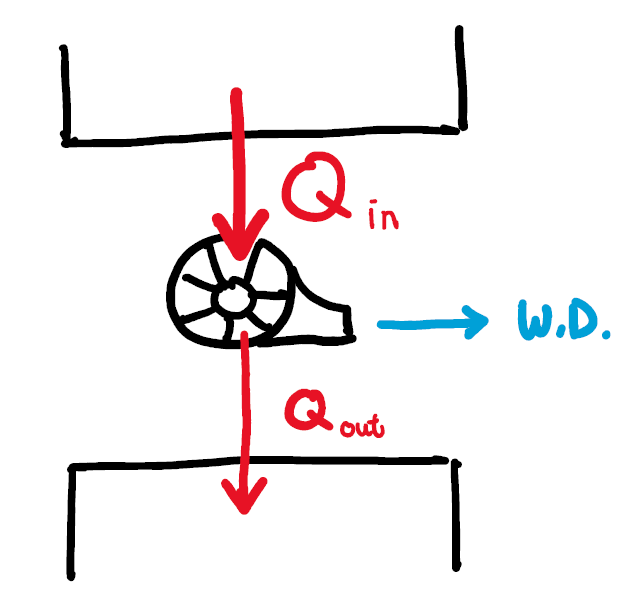
\includegraphics[width=\textwidth]{engine}
        \end{minipage}\\[1ex]
        %
        and\phantom{00000000000000000000}\\[1ex]
        %
        \begin{minipage}{0.78\linewidth}
            \aleq{
                \Aboxed{
                    \mstack{\text{Coefficient of}\\[0.3ex]\text{Performance}\\[0.3ex](\text{COP})} 
                    \ \defeq\  
                    \frac{\text{Heat remove}}{\text{W.D.}} 
                        = \qty|\frac{Q_\text{out}}{Q_\text{in}-Q_\text{out}}|
                        = \frac{1-\eta}{\eta}
                }
            }
        \end{minipage}
        \begin{minipage}{0.2\linewidth}
            \centering
            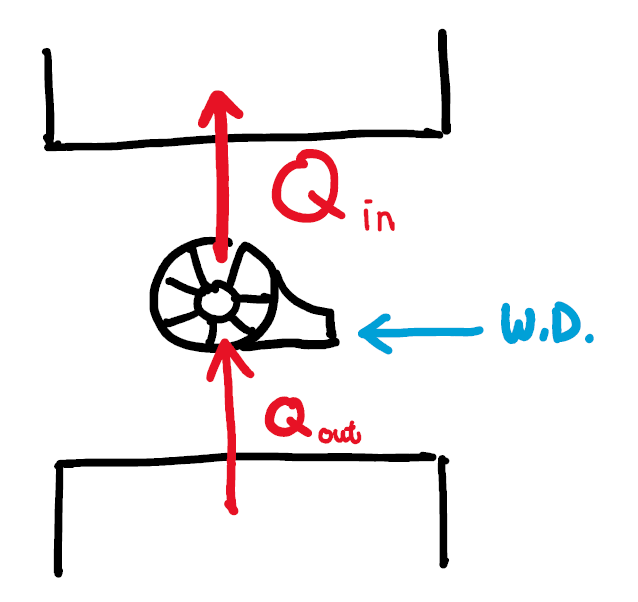
\includegraphics[width=\textwidth]{fridge}
        \end{minipage}
    \end{center}

    For example in the cycle with 4 processes, we can compute the efficiency as
    \aleq{
        \eta = 1 - \qty|\frac{\dfrac{i+2}{2}nR(T_4-T_3)}{\dfrac{i}{2}nR(T_1-T_4) + NT_1\ln\qty(\dfrac{V_2}{V_1})}|
    }
    
    \end{enumerate}

\end{example}

\vskip 1em
\begin{example}
    Thermal processes of photon gas \\

    This time we are dealing with a non-ideal gas material. 
    Photon gas' internal energy and pressure relation are given by
    \aleq{
        \bcase{
            U &= 3PV \blue{= \tkn{photon_U}{aVT^4}}\\
            P &= \frac{1}{3}aT^4
        }
        \quad\quad\quad
        \text{with }a = \text{some constant} 
    }
    \addBentArrow[blue]{photon_U}{(-5.5ex,-4.5ex)}
    {\scriptsize Substitute\\[-1ex]\scriptsize to get}{(0,-1ex)}{(10ex,1ex)}

    \gray{
        In comparison, we cannot use any properties of ideal gas, i.e. 
        $\bcase{
            U &= \frac{i}{2}PV = \frac{i}{2}nRT\\
            P &= \frac{nRT}{V}
        }$
    }

    \vskip 1em
    We have to re-derive $\dd{U}, \var{W}$ and $\var{Q}$ before we can proceed to solve any thermal cycle.

    \begin{enumerate}
        \item \ul{Internal Energy}\\
        Remember that $U$ is always a state function. 
        Its change is independent of process.
        \aleq{
            \Delta U &= U(P_2,V_2,T_2) - U(P_1,V_1,T_1)\\
            \Acboxed[green]{\Delta U &= 3(P_2V_2 - P_1V_1) = a(V_2T_2^4 - V_1T_1^4)}
        }

        \item \ul{Iso V.}\\
        By definition of the process, $\int \var{W}$ is always $0$. 
        Then for heat,
        \aleq{
            \Acboxed[green]{
                \int_\yellow{\text{iso. }V} \dd{Q} = \Delta U
                &= 3V(P_2 - P_1) = aV(T_2^4 - T_1^4)
            }
        } 

        The heat capacity under constant volume is then
        \aleq{
            \Acboxed[green]{
                \int C_\yellow{V} \dd{T} = \dvv{U}{T} = 4aVT^3 = (\text{NOT a constant})
            }
        }

        \item \ul{Iso P. and Iso T.}\\
        Note that in the pressure relation, $P = \inv{3}aT^4$, 
        \cul[red]{if $P$ is fixed, then $T$ is also fixed!}
        \aleq{
            \Acboxed[green]{\Delta U &= 3P(V_2-V_1) = aT^4(V_2-V_1)}\\
            \Acboxed[green]{\int_\yellow{\text{iso. }P} \var{W} &= P(V_2-V_1) = \frac{1}{3}aT^4(V_2-V_1)}\\
            \Acboxed[green]{\int_\yellow{\text{iso. }P} \var{Q} &= \Delta U + \int \var{W} = 4P(V_2-V_1) = \frac{4}{3}aT^4(V_2-V_1)}
        }

        However, it is impossible to define the heat capacity under constant pressure, 
        because you cannot change temperature under constant pressure.
        \aleq{
                \Acboxed[green]{
                \int_\yellow{\text{iso. }P} \var{Q} 
                = \int C_\yellow{P} \dd{T} 
                = \int (\text{undefined})\cdot (0)
            }
        }

        \item \ul{Adiabatic}\\
        By definition of the process, $\int \var{Q}$ is always $0$.
        Then we can derive the adiabatic relation:
        \aleq{
            P\dd{V} &= -\dd{U}\\
            &= -\dd{(3PV)} = -3(P\dd{V}+V\dd{P})\\
            4P\dd{V} &= -3V\dd{P}\\
            \frac{4}{3} \int \frac{\dd{V}}{V} &= -\int\frac{\dd{P}}{P}\\
            \ln(V^{\frac{4}{3}}) &= -\ln P + (\text{constant})\\
            \Acboxed[green]{
                PV^{\frac{4}{3}} &= (\text{constant})
            }
        }
        The adiabatic constant for photon gas is $\gamma =\dfrac{4}{3} \neq \dfrac{C_V}{C_P}$, obviously.

    \end{enumerate}

\end{example}

\vskip 2em
\begin{example}

    Carnot cycle by photon gas \\

    By definition, a Carnot cycle is made of 4 processes:

    \begin{center}
        \begin{minipage}{0.4\linewidth}
            \begin{enumerate}
                \item Iso. T (expansion)
                \item Adiabatic (expansion)
                \item Iso. T (contraction)
                \item Adiabatic (contraction)
            \end{enumerate}
        \end{minipage}
        \hspace{0.05\textwidth}
        \begin{minipage}{0.3\linewidth}
            \centering
            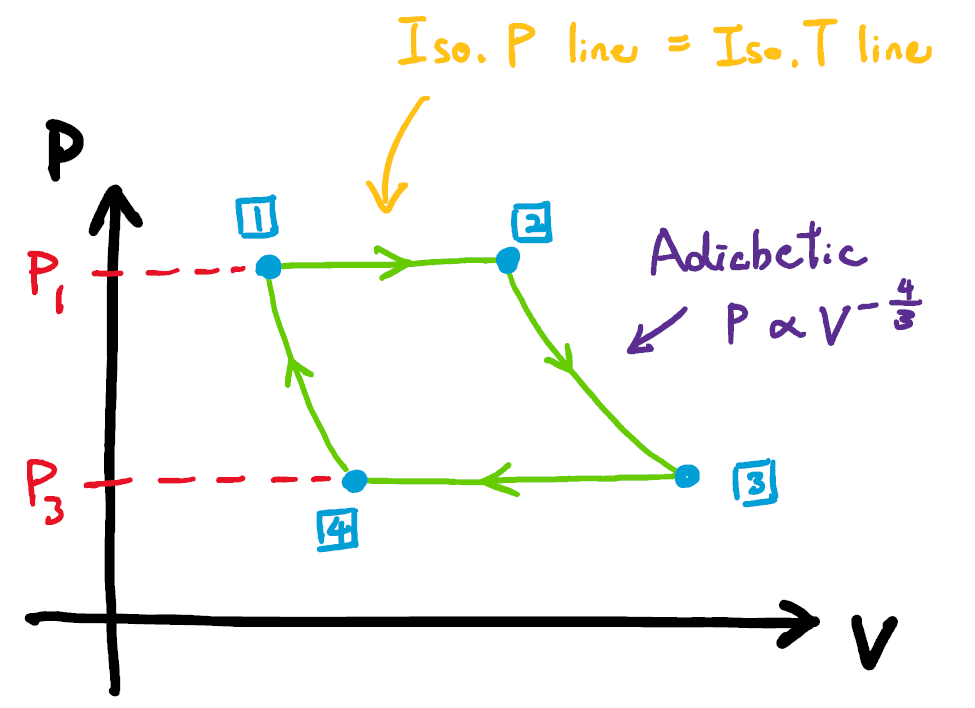
\includegraphics[width=\textwidth]{photon}
        \end{minipage}
    \end{center}

    \begin{enumerate}
        \item Write down the relations of $P,V,T$ between initial/final states of each process.
        \begin{center}
            \begin{minipage}{0.8\linewidth}
                \centering
                \begin{tabular}{>{\centering\arraybackslash}m{3cm} >{\centering\arraybackslash}m{3cm} >{\centering\arraybackslash}m{3cm}}
                    & Process & Relation
                    \\
                    \hline
                    \cbox[blue]{1} $\rightarrow$ \cbox[blue]{2}
                    & Iso. P \& T
                    & $P_1=P_2, T_1=T_2$
                    \\
                    \hline
                    \cbox[blue]{2} $\rightarrow$ \cbox[blue]{3}
                    & Adiabatic
                    & $P_2V_2^\gamma=P_3V_3^\gamma$
                    \\
                    \hline
                    \cbox[blue]{3} $\rightarrow$ \cbox[blue]{4}
                    & Iso. P \& T
                    & $P_3=P_4, T_3=T_4$
                    \\
                    \hline
                    \cbox[blue]{4} $\rightarrow$ \cbox[blue]{1}
                    & Adiabatic
                    & $P_4V_4^\gamma=P_1V_1^\gamma$
                \end{tabular}
            \end{minipage}
        \end{center}
        
    \item Write down the $\dd{U}, \var{W}, \var{Q}$ for each process.
    \begin{center}
        \begin{tabular}{>{\centering\arraybackslash}m{2cm} 
            >{\centering\arraybackslash}m{2.5cm} 
            c}
            & Process & $\dd{U},\var{Q},\var{W}$
            \\
            \hline
            \cbox[blue]{1} $\rightarrow$ \cbox[blue]{2}
            & Iso. P \& T
            & \makecell[l]{
                \phantom{\scriptsize abc}\\
                $\bcase{
                    \Delta U &= aT_1^4(V_2-V_1)\\
                    \int \var{W} &= \inv{3} aT_1^4(V_2-V_1)\\
                    \int \var{Q} &= \frac{4}{3}aT_1^4(V_2-V_1) \quad \red{>0}\\
                }$\\
                \phantom{\scriptsize abc}
            }
            \\
            \hline
            \cbox[blue]{2} $\rightarrow$ \cbox[blue]{3}
            & Adiabatic
            & \makecell[l]{
                \phantom{\scriptsize abc}\\
                $\bcase{
                    \Delta U &= a(V_3T_3^4-V_2T_2^4)\\
                    \int \var{W} &= -a(V_3T_3^4-V_2T_2^4)\\
                    \int \var{Q} &= 0\\
                }$\\
                \phantom{\scriptsize abc}
            }
            \\
            \hline
            \cbox[blue]{3} $\rightarrow$ \cbox[blue]{4}
            & Iso. P
            & \makecell[l]{
                \phantom{\scriptsize abc}\\
                $\bcase{
                    \Delta U &= aT_3^4(V_4-V_3)\\
                    \int \var{W} &= \inv{3} aT_3^4(V_4-V_3)\\
                    \int \var{Q} &= \frac{4}{3}aT_3^4(V_4-V_3) \quad \red{<0}\\
                }$\\
                \phantom{\scriptsize abc}
            }
            \\
            \hline
            \cbox[blue]{4} $\rightarrow$ \cbox[blue]{1}
            & Iso. V
            & \makecell[l]{
                \phantom{\scriptsize abc}\\
                $\bcase{
                    \Delta U &= a(V_1T_1^4-V_4T_4^4)\\
                    \int \var{W} &= -a(V_1T_1^4-V_4T_4^4)\\
                    \int \var{Q} &= 0\\
                }$\\
                \phantom{\scriptsize abc}
            }
        \end{tabular}
    \end{center}

    \item Identify if the $\var{Q}$ of each process is an input or output.
    We can check for each process,
    \begin{itemize}
        \item With heat input: \cbox[blue]{1} $\rightarrow$ \cbox[blue]{2}
        \item With heat output: \cbox[blue]{3} $\rightarrow$ \cbox[blue]{4}
    \end{itemize}


    \item Calculate efficiency according to the signs of $\var{Q}$.
    \aleq{
        \Aboxed{
            \eta
            = 1- \qty|\frac{\text{Heat output}}{\text{Heat intput}}|
            = 1-\qty|\frac{\ccancel[red]{\dfrac{4}{3}a}T_3^4(V_4-V_3)}{\ccancel[red]{\dfrac{4}{3}a}T_1^4(V_2-V_1)}|
        }
    }

    To simplify, we can use the adiabatic relation:
    \aleq{
        PV^{\frac{4}{3}} &= (\text{const.})\\
        \Rightarrow\ \inv{3}aT^4V^{\frac{4}{3}} &= (\text{const.})\\
        \Rightarrow\qquad T^3V &= (\text{const.})
    }

    And the relations between state parameters that we derived in step 1:
    \aleq{
        \bcase{
            & T_1=T_2,\  T_3=T_4\\
            & T_2^3V_2 = T_3^3V_3,\  T_4^3V_4=T_1^3V_1
        }
    }

    The efficiency is now
    \aleq{
        \eta
        &= 1- \qty|\frac{T_3^4(V_4-V_3)}{T_1^4(V_2-V_1)}| \\[1ex]
        &= 1- \frac{T_3}{T_1}\qty|\frac{T_3^3V_4 - T_3^3V_3}{T_1^3V_2 - T_1^3V_1}|\\[1ex]
        &= 1- \frac{T_3}{T_1}\qty|\frac{T_\red{4}^3V_4 - T_3^3V_3}{T_\red{2}^3V_2 - T_1^3V_1}|\\[1ex]
        &= 1- \frac{T_3}{T_1}
    }

    which is exactly the same as Carnot cycle with ideal gas!

    \end{enumerate}

\end{example}




%%%
\theend
\end{document}